\documentclass{article}
\usepackage[left=1in,right=1in,top=1in,bottom=1in]{geometry}
\usepackage{amsmath, amsthm, verbatim, enumerate, totcount}
\usepackage[usenames,dvipsnames]{xcolor}
\usepackage{enumerate, tikz, booktabs}
\usepackage{wrapfig}
\usepackage{hyperref}
\usepackage{mathpartir}
\usepackage{listings}
\usepackage{fancyhdr}
\usepackage{pythonhighlight}
\usepackage{graphicx}
\usetikzlibrary{automata,positioning,arrows}


\pagestyle{fancy}
\fancyhf{}
\rhead{My Dinh}
\lhead{CS 458: Introduction to Information Security}
\cfoot{\thepage}

\setlength\parindent{0pt}
\setlength{\parskip}{1em}
\renewcommand{\thesubsection}{\thesection.\arabic{subsection}}

\title{IIT CS458: Introduction to Information Security\\
  {\large Homework 3: MD5 Collision Attack Lab}}
\author{My Dinh}
\date{}

\begin{document}
\maketitle

\addtocounter{section}{1}

\section{Lab Tasks}

\subsection{Task 1: Generating Two Different Files with the Same MD5 Hash}

In this task, I wrote a Python program to generate a string with the size in
bytes given by the user in the command line interface.

\begin{python}
import sys

char = "6"
length = sys.argv[1]
sentence = char * int(length)

print(sentence)
\end{python}

\lstset{basicstyle=\footnotesize\ttfamily,
  showstringspaces=false,
  commentstyle=\color{gray},
  keywordstyle=\color{blue},
  frame=single,
  rulecolor=\color{gray}
}

The bash script below is for generating the \texttt{out1.bin} and \texttt{out2.bin}
files using \texttt{md5collgen}, comparing their hex using \texttt{hexdump} and
\texttt{diff}, and checking their \texttt{md5sum} from the \texttt{prefix.txt}
file in question 1 and 2 of task 1.

\begin{lstlisting}[language=bash]
#!/bin/sh


generate_md5() {
    echo -n $(python3 generate_string.py $1) > prefix.txt
    echo "+ prefix.txt content: $(cat prefix.txt)"
    echo "+ Size of prefix.txt: $(wc -c < prefix.txt) bytes"

    echo "\n+ Running md5collgen"
    md5collgen -p prefix.txt -o out1.bin out2.bin --quiet

    echo
    echo "+ Size of out1.bin: $(wc -c < out1.bin) bytes"
    echo "+ Size of out2.bin: $(wc -c < out2.bin) bytes"

    echo "\n+ Check diff out1.bin out2.bin"
    diff out1.bin out2.bin -q

    echo "\n+ View md5sum out1.bin and out2.bin"
    md5sum out1.bin
    md5sum out2.bin

    echo "\n+ Compare out1.bin and out2.bin hex"
    echo "out1.bin"
    hexdump out1.bin
    echo "\nout2.bin"
    hexdump out2.bin
}

question_1() {
    echo "\nQuestion 1"
    generate_md5 69
}

question_1

question_2
\end{lstlisting}

\textbf{Question 1.} If the length of the \texttt{prefix.txt} file is not multiple
of 64 (in this case, my \texttt{prefix.txt} file is 69 bytes), the binary files
\texttt{out1.bin} and \texttt{out2.bin} generated by \texttt{md5collgen} would
have padding at the beginning of the hex of the file. We can check this by using
\texttt{hexdump} tool.

\begin{figure}[!ht]
    \centering
    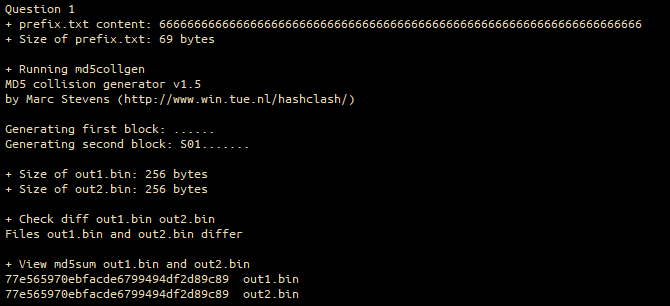
\includegraphics[scale=0.5]{task1.1.1.png}
    \caption{Size and md5sum of out1.bin and out2.bin for 69 byte prefix file.}
\end{figure}

\begin{figure}[!ht]
    \centering
    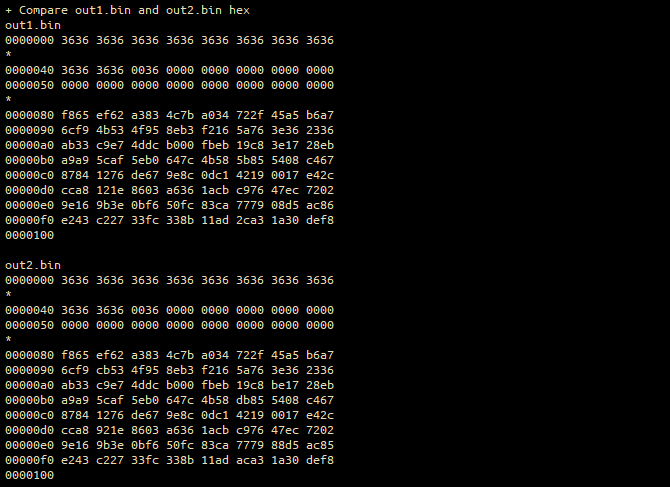
\includegraphics[scale=0.5]{task1.1.2.png}
    \caption{Hexdump of out1.bin and out2.bin for 69 byte prefix file.}
\end{figure}

\textbf{Question 2.} If the \texttt{prefix.txt} file is exactly 64 bytes the the
result files \texttt{out1.bin} and \texttt{out2.bin} do not have padding at the
beginning of the files. The size of both binary files are 192 bytes.

\begin{figure}[!ht]
    \centering
    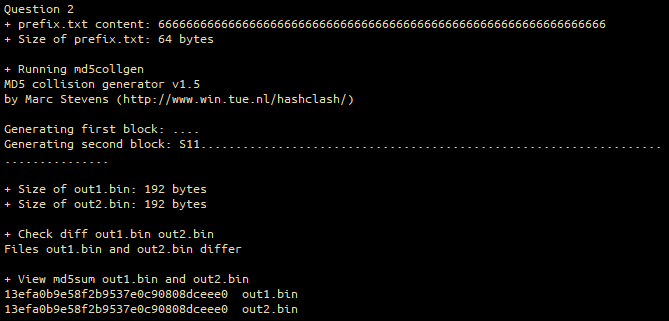
\includegraphics[scale=0.5]{task1.2.1.png}
    \caption{Size and md5sum of out1.bin and out2.bin for 64 byte prefix file.}
\end{figure}

\begin{figure}[!ht]
    \centering
    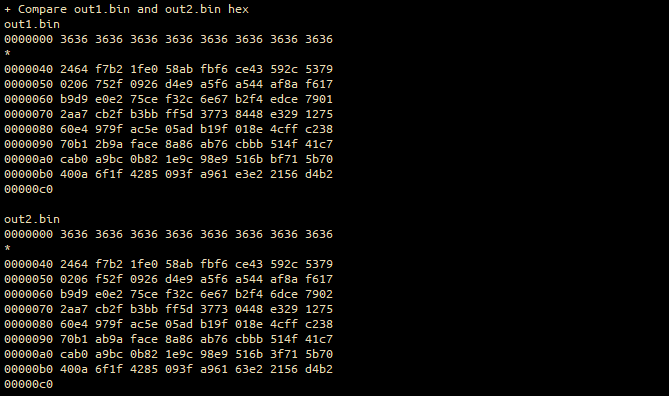
\includegraphics[scale=0.5]{task1.2.2.png}
    \caption{Hexdump of out1.bin and out2.bin for 64 byte prefix file.}
\end{figure}

\textbf{Question 3.} For this question, I'm going to use the result output files
for 64 byte \texttt{prefix.txt} file.

\begin{lstlisting}[language=bash]
#!/bin/sh

question_3() {
    echo "\nQuestion 3"
    tail -c 128 out1.bin > data1
    tail -c 128 out2.bin > data2
    diff data1 data2 -q
}

question_3
\end{lstlisting}

The code snippet above would store the last 128 bytes of \texttt{out1.bin} in
\texttt{data1} file and the last 128 bytes of \texttt{out2.bin} in \texttt{data2}.
I then used \texttt{diff} to check if the data of generated by \texttt{md5collgen}
were different. The result of the code snippet was \texttt{"Files data1 and data2 differ"},
meaning that \texttt{data1} and \texttt{data2} did not contain the same data.

To find all the different bytes in \texttt{data1} and \texttt{data2}, I had written
the following program in Python to compare the bytes of each file.

\begin{python}
with open("data1", "rb") as f:
    hex1 = f.read()

with open("data2", "rb") as f:
    hex2 = f.read()

for i in range(len(hex1)):
    if hex1[i] != hex2[i]:
        print(f'Diff hex value at position {hex(i)} in data1 and data2: {hex(hex1[i])} {hex(hex2[i])}')
\end{python}

The result can be found in Figure \ref{fig:task1_question3_result}.

\begin{figure}[!ht]
    \centering
    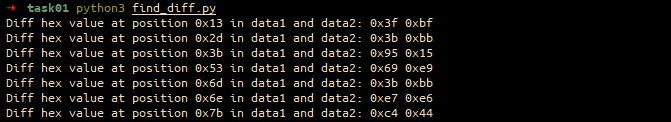
\includegraphics[scale=0.5]{task1.3.1.png}
    \caption{Different bytes in the 128 bytes generated by md5collgen in out1.bin and out2.bin.}
    \label{fig:task1_question3_result}
\end{figure}

\subsection{Task 2: Understanding MD5's Property}

For this task, first I generated two different files that have the same md5sum
using \texttt{md5collgen} and stored them in \texttt{out1.bin} and \texttt{out2.bin}
respectively.

\begin{figure}[!ht]
    \centering
    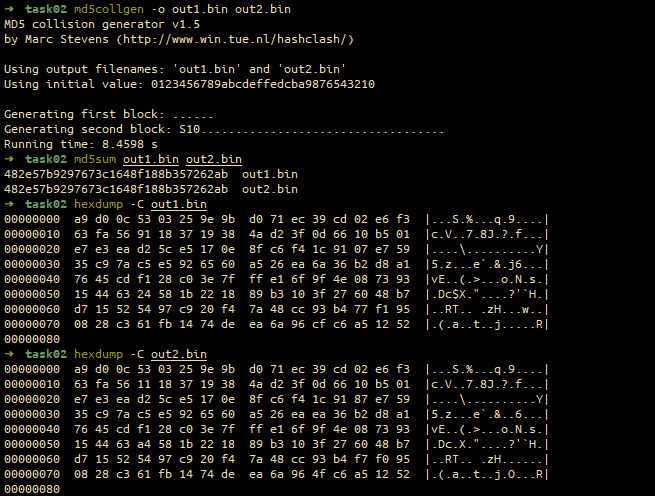
\includegraphics[scale=0.5]{task2.1.png}
    \caption{Generating different files with the same MD5 hash.}
\end{figure}

I then created a file that contains extra text \texttt{"extra text"}, added it to the
end of \texttt{out1.bin} and \texttt{out2.bin} to create \texttt{extra1} and
\texttt{extra2} file, and checked the md5 hash value of the new file using
\texttt{md5sum}.

\begin{figure}[!ht]
    \centering
    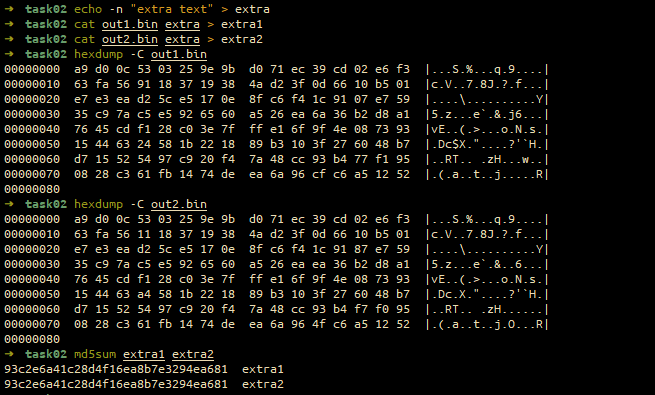
\includegraphics[scale=0.5]{task2.2.png}
    \caption{Comparing MD5 hash of new files.}
\end{figure}

From the result of \texttt{hexdump}, I could conclude that the same data was
concatenated at the end of both \texttt{out1.bin} and \texttt{out2.bin}.
The MD5 hash generated from \texttt{md5sum} tool of new files \texttt{extra1}
and \texttt{extra2}, which were \texttt{out1.bin} and \texttt{out2.bin} with the
message \texttt{"extra text"} added to the end of the file, are the same (both
are equal to \texttt{"93c2e6a41c28d4f16ea8b7e3294ea681"}).

\subsection{Task 3: Generating Two Executable Files with the Same MD5 Hash}

The content of the C program I used for this task is

\begin{lstlisting}[language=c]
#include <stdio.h>

unsigned char xyz[200] = {
    0x41,0x41,0x41,0x41,0x41,0x41,0x41,0x41,0x41,0x41,0x41,0x41,0x41,0x41,0x41,
    0x41,0x41,0x41,0x41,0x41,0x41,0x41,0x41,0x41,0x41,0x41,0x41,0x41,0x41,0x41,
    0x41,0x41,0x41,0x41,0x41,0x41,0x41,0x41,0x41,0x41,0x41,0x41,0x41,0x41,0x41,
    0x41,0x41,0x41,0x41,0x41,0x41,0x41,0x41,0x41,0x41,0x41,0x41,0x41,0x41,0x41,
    0x41,0x41,0x41,0x41,0x41,0x41,0x41,0x41,0x41,0x41,0x41,0x41,0x41,0x41,0x41,
    0x41,0x41,0x41,0x41,0x41,0x41,0x41,0x41,0x41,0x41,0x41,0x41,0x41,0x41,0x41,
    0x41,0x41,0x41,0x41,0x41,0x41,0x41,0x41,0x41,0x41,0x41,0x41,0x41,0x41,0x41,
    0x41,0x41,0x41,0x41,0x41,0x41,0x41,0x41,0x41,0x41,0x41,0x41,0x41,0x41,0x41,
    0x41,0x41,0x41,0x41,0x41,0x41,0x41,0x41,0x41,0x41,0x41,0x41,0x41,0x41,0x41,
    0x41,0x41,0x41,0x41,0x41,0x41,0x41,0x41,0x41,0x41,0x41,0x41,0x41,0x41,0x41,
    0x41,0x41,0x41,0x41,0x41,0x41,0x41,0x41,0x41,0x41,0x41,0x41,0x41,0x41,0x41,
    0x41,0x41,0x41,0x41,0x41,0x41,0x41,0x41,0x41,0x41,0x41,0x41,0x41,0x41,0x41,
    0x41,0x41,0x41,0x41,0x41,0x41,0x41,0x41,0x41,0x41,0x41,0x41,0x41,0x41,0x41,
    0x41,0x41,0x41,0x41,0x41

};

int main() {
    int i;
    for (i = 0; i < 200; i++)
        printf("%x", xyz[i]);
    printf("\n");
}
\end{lstlisting}

I made array \texttt{xyz} to contain 200 character A's so it would be easier for
me to locate the array in the binary file after compiling the C program above.

To locate the position of array \texttt{xyz} in the binary file without using
\texttt{bless} (because I don't have \texttt{bless} installed in my local machine),
I wrote a Python program to go through the bytes and pin point the start and the
end position of the array in the executable file.

\begin{python}
with open("a.out", "rb") as f:
    byte_stream = f.read()
f.close()


# find the start and end byte block of the xyz array that contains 200 A's
def find_A_range():
    start, end = 0, 0
    for i in range(len(byte_stream)):
        if byte_stream[i] == 0x41:
            start = i
            end = i

            while end < len(byte_stream) and byte_stream[end] == 0x41:
                end += 1

            end -= 1

            if end - start + 1 == 200:
                break

    return (start, end)


# get the size of prefix
def get_prefix_size(start: int) -> int:
    return start + (64 - start % 64)


# get the size of prefix
def get_suffix_size(prefix_size: int) -> int:
    return len(byte_stream) - prefix_size - 128


if __name__ == "__main__":
    start, _ = find_A_range()
    prefix_size = get_prefix_size(start)
    suffix_size = get_suffix_size(prefix_size)

    print(prefix_size, suffix_size)
\end{python}

Using that information, I created two functions to get the size of the \texttt{prefix}
and \texttt{suffix} file. To do this, the function \texttt{get\_prefix\_size}
finds a multiple of \texttt{64} that is nearest to the value of start position.
And the suffix size is found by calculating the difference between the size of
the executable and the size of prefix and \texttt{128}.

Finally, I wrote a bash script to run all the commands to generate \texttt{a1.out}
and \texttt{a2.out} which are the two executable files with the same MD5 hash
but have different elements in array \texttt{xyz}.

\begin{lstlisting}[language=bash]
#!/bin/sh

# get prefix and suffix file using the given sizes
get_prefix_and_suffix() {
    PREFIX_SIZE=$1
    SUFFIX_SIZE=$2

    echo "prefix size: ${PREFIX_SIZE}, suffix size: ${SUFFIX_SIZE}"
    head -c $PREFIX_SIZE a.out > prefix
    tail -c $SUFFIX_SIZE a.out > suffix
}

# compile and create executable file for the given C program
gcc array.c

# get prefix and suffix from the result size of prefix_suffix_size program
echo "+ Get prefix and suffix size"
get_prefix_and_suffix $(python3 prefix_suffix_size.py)

# generate P and Q with the same md5 hash
echo "\n+ Generating P and Q using prefix as prefixfile"
md5collgen -p prefix -o P Q

# create new executable files a1.out and a2.out using the new generated prefix
# P and Q
cat P suffix > a1.out
cat Q suffix > a2.out

echo "\n+ Check a1.out and a2.out md5 hash"
md5sum a1.out a2.out

echo "\n+ Compare a1.out and a2.out"
diff a1.out a2.out

echo "\n+ Execute a1.out"
./a1.out > array1
cat array1

echo "\n+ Execute a2.out"
./a2.out > array2
cat array2

echo "\n+ Compare the array in a1.out and a2.out"
diff -q array1 array2
\end{lstlisting}

The result can be found in Figure \ref{fig:task3_result}.

\begin{figure}[!ht]
    \centering
    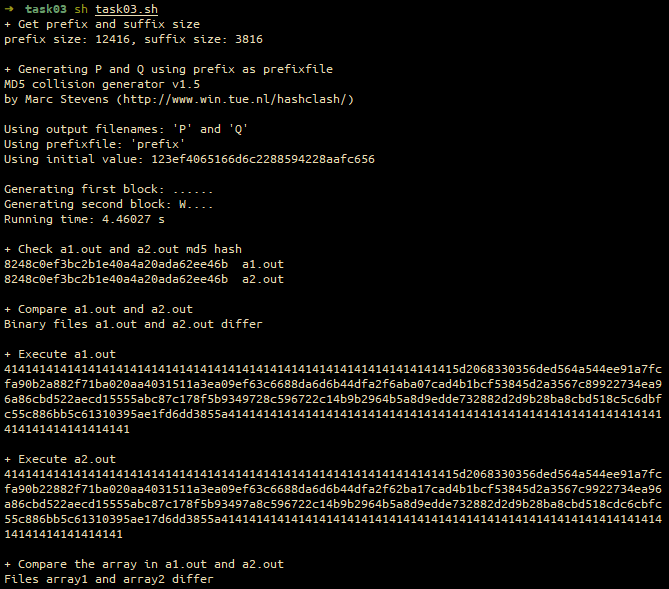
\includegraphics[scale=0.5]{task3.png}
    \caption{Result of new executable files a1.out and a2.out.}
    \label{fig:task3_result}
\end{figure}

From Figure \ref{fig:task3_result}, we can see that the new executable files
\texttt{a1.out} and \texttt{a2.out} have the same MD5 hash value
\texttt{8248c0ef3bc2b1e40a4a20ada62ee46b}, but contents of their \texttt{xyz}
array are different (this can be checked by storing the result of \texttt{./a1.out}
and \texttt{./a2.out} in two text files and comparing them using \texttt{diff} tool).

\subsection{Task 4: Making the Two Programs Behave Differently}

The content of the benign program I used for this task is

\begin{lstlisting}[language=c]
#include <stdio.h>

unsigned char X[200] = {
    0x41,0x41,0x41,0x41,0x41,0x41,0x41,0x41,0x41,0x41,0x41,0x41,0x41,0x41,0x41,
    0x41,0x41,0x41,0x41,0x41,0x41,0x41,0x41,0x41,0x41,0x41,0x41,0x41,0x41,0x41,
    0x41,0x41,0x41,0x41,0x41,0x41,0x41,0x41,0x41,0x41,0x41,0x41,0x41,0x41,0x41,
    0x41,0x41,0x41,0x41,0x41,0x41,0x41,0x41,0x41,0x41,0x41,0x41,0x41,0x41,0x41,
    0x41,0x41,0x41,0x41,0x41,0x41,0x41,0x41,0x41,0x41,0x41,0x41,0x41,0x41,0x41,
    0x41,0x41,0x41,0x41,0x41,0x41,0x41,0x41,0x41,0x41,0x41,0x41,0x41,0x41,0x41,
    0x41,0x41,0x41,0x41,0x41,0x41,0x41,0x41,0x41,0x41,0x41,0x41,0x41,0x41,0x41,
    0x41,0x41,0x41,0x41,0x41,0x41,0x41,0x41,0x41,0x41,0x41,0x41,0x41,0x41,0x41,
    0x41,0x41,0x41,0x41,0x41,0x41,0x41,0x41,0x41,0x41,0x41,0x41,0x41,0x41,0x41,
    0x41,0x41,0x41,0x41,0x41,0x41,0x41,0x41,0x41,0x41,0x41,0x41,0x41,0x41,0x41,
    0x41,0x41,0x41,0x41,0x41,0x41,0x41,0x41,0x41,0x41,0x41,0x41,0x41,0x41,0x41,
    0x41,0x41,0x41,0x41,0x41,0x41,0x41,0x41,0x41,0x41,0x41,0x41,0x41,0x41,0x41,
    0x41,0x41,0x41,0x41,0x41,0x41,0x41,0x41,0x41,0x41,0x41,0x41,0x41,0x41,0x41,
    0x41,0x41,0x41,0x41,0x41

};

unsigned char Y[200] = {
    0x41,0x41,0x41,0x41,0x41,0x41,0x41,0x41,0x41,0x41,0x41,0x41,0x41,0x41,0x41,
    0x41,0x41,0x41,0x41,0x41,0x41,0x41,0x41,0x41,0x41,0x41,0x41,0x41,0x41,0x41,
    0x41,0x41,0x41,0x41,0x41,0x41,0x41,0x41,0x41,0x41,0x41,0x41,0x41,0x41,0x41,
    0x41,0x41,0x41,0x41,0x41,0x41,0x41,0x41,0x41,0x41,0x41,0x41,0x41,0x41,0x41,
    0x41,0x41,0x41,0x41,0x41,0x41,0x41,0x41,0x41,0x41,0x41,0x41,0x41,0x41,0x41,
    0x41,0x41,0x41,0x41,0x41,0x41,0x41,0x41,0x41,0x41,0x41,0x41,0x41,0x41,0x41,
    0x41,0x41,0x41,0x41,0x41,0x41,0x41,0x41,0x41,0x41,0x41,0x41,0x41,0x41,0x41,
    0x41,0x41,0x41,0x41,0x41,0x41,0x41,0x41,0x41,0x41,0x41,0x41,0x41,0x41,0x41,
    0x41,0x41,0x41,0x41,0x41,0x41,0x41,0x41,0x41,0x41,0x41,0x41,0x41,0x41,0x41,
    0x41,0x41,0x41,0x41,0x41,0x41,0x41,0x41,0x41,0x41,0x41,0x41,0x41,0x41,0x41,
    0x41,0x41,0x41,0x41,0x41,0x41,0x41,0x41,0x41,0x41,0x41,0x41,0x41,0x41,0x41,
    0x41,0x41,0x41,0x41,0x41,0x41,0x41,0x41,0x41,0x41,0x41,0x41,0x41,0x41,0x41,
    0x41,0x41,0x41,0x41,0x41,0x41,0x41,0x41,0x41,0x41,0x41,0x41,0x41,0x41,0x41,
    0x41,0x41,0x41,0x41,0x41

};

int compare(unsigned char *X, unsigned char *Y) {
    int i;
    for (i = 0; i < 200; i++) {
        if (X[i] != Y[i])
            return 0;
    }
    return 1;
}

int main() {

    int i;

    printf("X = ");
    for (i = 0; i < 200; i++)
        printf("%x", X[i]);
    printf("\n");

    printf("Y = ");
    for (i = 0; i < 200; i++)
        printf("%x", Y[i]);
    printf("\n");

    if (compare(X, Y))
        printf("\nDo something good :)");
    else
        printf("\nDo something bad >:)");
    printf("\n");
}
\end{lstlisting}

When executed, the program will print the elements in \texttt{X} and \texttt{Y}
array. If the the arrays are equal, it will print out \texttt{"Do something good :)"},
else print \texttt{"Do something bad >:)"}.

In this task, I wrote a Python program to apply the method mentioned in the instruction
to create a program include malicious code that has the same MD5 hash with the
benign one.

\begin{python}
from subprocess import run

with open("a.out", "rb") as f:
    BYTE_STREAM = f.read()
f.close()


# get the starting and ending position of X and Y in the byte stream
def get_X_Y_location(byte_stream):
    start_end = []
    for i in range(len(byte_stream)):
        if byte_stream[i] == 0x41:
            start = i
            end = i
            while end < len(byte_stream) and byte_stream[end] == 0x41:
                end += 1
            end -= 1
            if end - start + 1 == 200:
                start_end.append((start, end))
    return start_end


# get the offset of the array in the byte stream
def get_array_offset(start: int) -> int:
    return 64 - start % 64


# get the prefix size
def get_prefix_size(start: int, offset: int) -> int:
    return start + offset


# get the suffix size
def get_suffix_size(byte_stream_size: int, prefix_size: int) -> int:
    return byte_stream_size - 128 - prefix_size


# clean file in the current directory
def clean():
    run('rm -rf prefix* suffix* P Q a1.out a2.out', shell=True)


if __name__ == "__main__":

    start_end = get_X_Y_location(BYTE_STREAM)

    s1, e1 = start_end[0]
    s2, e2 = start_end[1]

    offset = get_array_offset(s1)
    prefix_size = get_prefix_size(s1, offset)
    suffix_size = get_suffix_size(len(BYTE_STREAM), prefix_size)

    try:
        clean()
    except Exception:
        pass

    # get the prefix and the suffix of the executable file
    run(f'head -c {prefix_size} a.out > prefix', shell=True)
    run(f'tail -c {suffix_size} a.out > suffix', shell=True)

    # generate two files with the same md5 using prefix as prefixfile
    print("\n+ Generate prefix_P and prefix_Q")
    run('md5collgen -p prefix -o prefix_P prefix_Q', shell=True)

    # get P and Q (the 128 bytes generate by md5collgen) from prefix_P and prefix_Q
    run('tail -c 128 prefix_P > P', shell=True)
    run('tail -c 128 prefix_Q > Q', shell=True)

    # get the starting position of Y with offset relative to starting position
    # of suffix
    # get the end position of 128 bytes from the starting position of Y with
    # offset
    s2_P = s2 - 128 - prefix_size + offset
    e2_P = s2_P + 128

    # insert P in the middle of array Y in the suffix
    run(f'head -c {s2_P} suffix > suffix_pre', shell=True)
    run(f'tail -c +{e2_P} suffix > suffix_post', shell=True)
    run('cat suffix_pre P suffix_post > suffix_P', shell=True)

    # concat prefix_p and prefix_Q with suffix_P to create two new executable
    # files a1.out and a2.out with the same md5 hash
    run('cat prefix_P suffix_P > a1.out', shell=True)
    run('cat prefix_Q suffix_P > a2.out', shell=True)

    # compare md5 hash of a1.out and a2.out
    print("\n+ Compare a1.out and a2.out md5 hash")
    run('md5sum a1.out a2.out', shell=True)

    # execute a1.out and a2.out
    print("\n+ Result of program a1.out")
    run('./a1.out')

    print("\n+ Result of program a2.out")
    run('./a2.out')
\end{python}

The program uses the same method in Task 3 to find the position (starting
and ending index) of the target arrays and calculate the prefix and suffix size.
The different is I created another function to find the \texttt{offset}, which
is the extra bytes from the nearest multiple of 64 to create a prefix to the
starting position of array \texttt{X} in the executable file (the \texttt{offset}
will be useful later). The definiion of offset is shown in Figure \ref{fig:task4_offset}.

\begin{figure}[!ht]
    \centering
    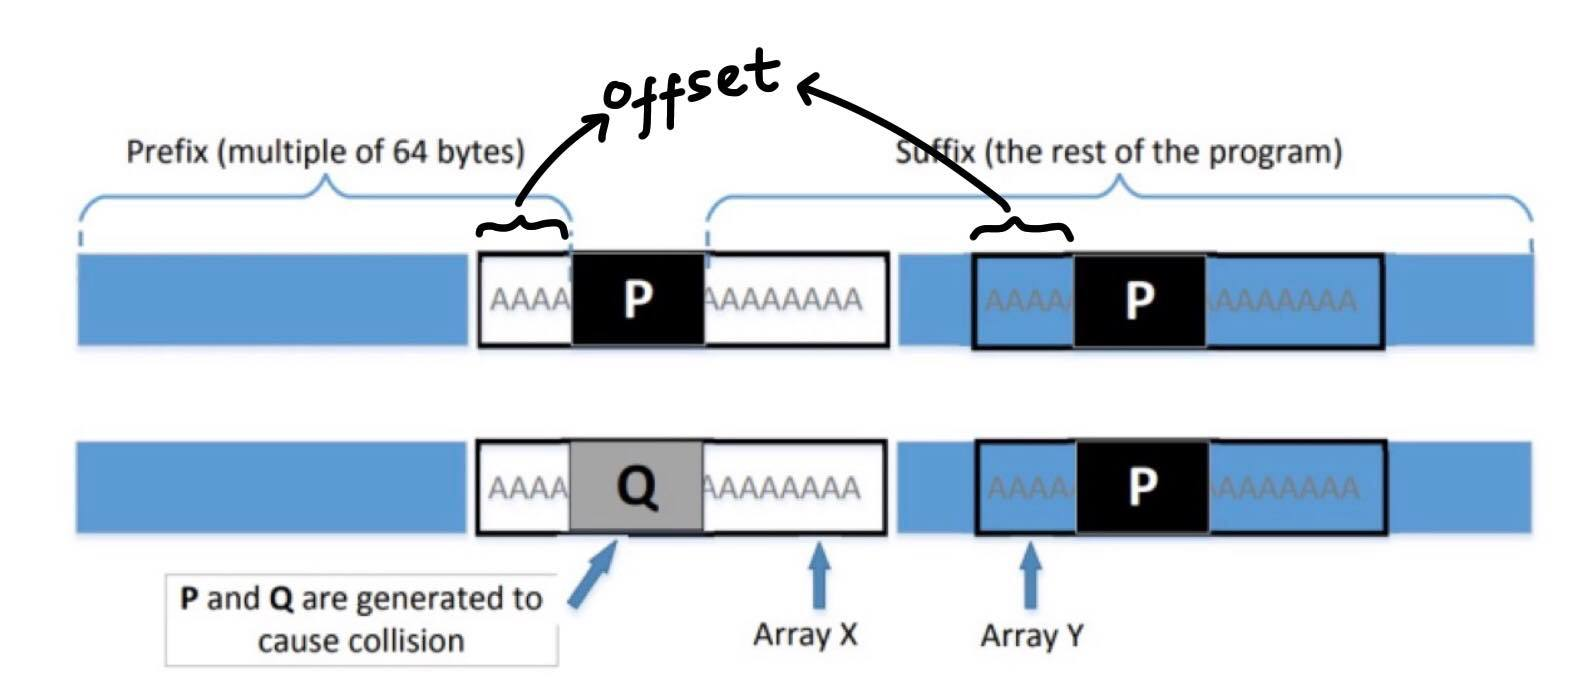
\includegraphics[scale=0.25]{task4.1.jpg}
    \caption{Offset of array X and Y.}
    \label{fig:task4_offset}
\end{figure}

After getting the \texttt{prefix} and \texttt{suffix}, I used \texttt{md5collgen}
with \texttt{prefix} as prefixfile to generate two new prefixes \texttt{prefix\_P}
and \texttt{prefix\_Q} with the same MD5 hash. Since we have to replace \texttt{P}
(the extra 128 bytes that \texttt{md5collgen} generated with \texttt{prefix} in
the new file) in the array \texttt{Y} like in \texttt{X}, I "cut" the \texttt{suffix}
file into two parts: the first part \texttt{suffix\_pre} is from the beginning of the \texttt{suffix}
to the starting position we have to insert \texttt{P}, the second one \texttt{suffix\_post}
is from the starting position to insert \texttt{P} plus 128 (because the size of
\texttt{P} is 128 bytes) to the end of \texttt{suffix}. Then I used \texttt{cat}
to concatenate \texttt{suffix\_pre}, \texttt{P}, and \texttt{suffix\_post} to
create a new suffix file \texttt{suffix\_P}.

The final step is to add the prefix and the suffix together to create new executable
files that have same MD5 has and contain malicious code: \texttt{a1.out} contains \texttt{P}
in both array \texttt{X} and \texttt{Y}, and \texttt{a2.out} contains \texttt{Q} in \texttt{X}
and \texttt{P} in \texttt{Y}. Since in \texttt{a1.out}, \texttt{X} and \texttt{Y}
have the same elements, it would run the benign code, while in \texttt{a2.out},
it would run the malicious code because \texttt{X} and \texttt{Y} are different.

Running the Python program above would give the result in Figure \ref{fig:task4_result}.

\begin{figure}[!ht]
    \centering
    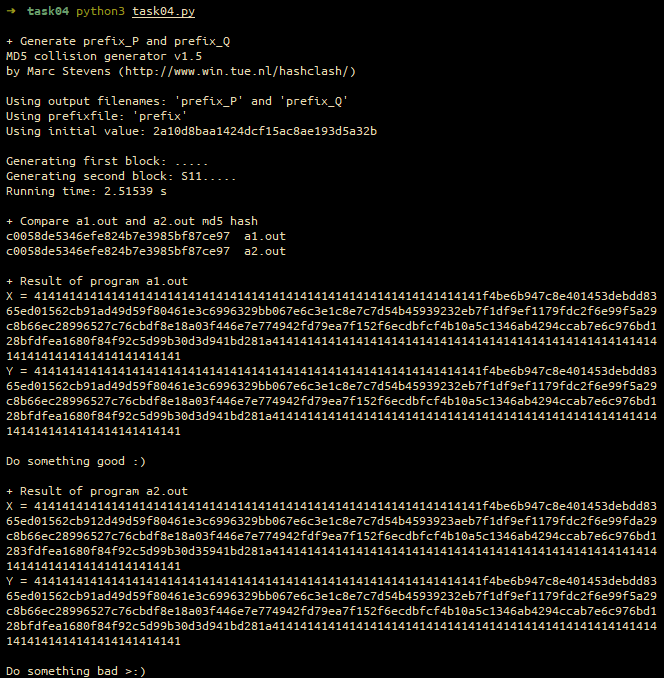
\includegraphics[scale=0.5]{task4.2.png}
    \caption{Two programs with the same MD5 hash behave Differently.}
    \label{fig:task4_result}
\end{figure}

As we suspected, \texttt{a1.out} ran the benign code which print out \texttt{"Do
something good :)"} and \texttt{a2.out} executed the malicious one and print
\texttt{"Do something bad >:)"}. Both programs have the same MD5 hash, which is
equal to \texttt{c0058de5346efe824b7e3985bf87ce97}.

\end{document}
